


\begin{algorithm}
\SetAlgoLined
    OPEN $\gets$ initial\\
    $g($initial.head$)\gets 0$\\
    CLOSED $\gets \emptyset$\\
    \While{OPEN is not empty}{
        current $\gets$ pop best node from OPEN\\
        Add current to CLOSED\\
        \If{current is a goal state}{
            \Return current
        }
        \ForEach{operator $o$ applicable in current \nllabel{line:astar:for}}{
            child $\gets$ apply $o$ on current\\
            newg $\gets$ $g($current.head$)$+ cost($o$)\\
            \HiLi \If{$\exists$n$\in$OPEN$\cup$CLOSED s.t. $n.$head=child.head}{
                \HiLi \eIf{$g($child.head$)\leq$newg}{
                    \HiLi Goto line~\ref{line:astar:for}\\
                }{
                    \HiLi Remove(n,OPEN)\\
                }
            }
            $g($child.head$)\gets$newg\\
            \HiLi Insert$\Big($child, $g($child.head$)+h($child$)\Big)$\\
        }
    }
    \Return no solution found
 \caption{The A* Algorithm}
 \label{alg:astar}
\end{algorithm}



A state space is said to be \emph{monotone} w.r.t a start state $s$ 
and an optimization criteria if for any path $\pi$ in the state space starting from $s$ it holds that $\pi$ is not better than any prefix of $\pi$, where better is defined by the chosen optimization criteria~\cite{DBLP:conf/socs/SternKPFR14}. In SP, the relevant optimization criteria is to find the shortest path while in LSP the relevant optimization criteria is to find the longest path. With respect to these optimization criteria, it is easy to see that the SP state space is monotone for every start state while the LSP state space is not. For example, consider Figure \ref{fig:optimal_sub_structure}. If if we're looking for the longest path from verex $s$ to vertex $t$ it will be $[s,a,t]$. But the longest path from vertex $s$ to vertex $a$ is $[s,b,t,a]$.

\begin{figure}
\centering
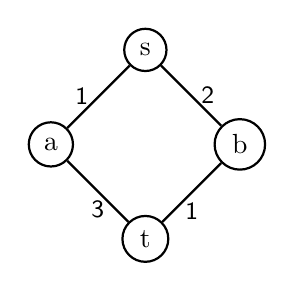
\begin{tikzpicture}[auto, node distance=1.2cm,
                    thick,main node/.style={circle,draw}]

  \node[main node] (0) {s};
  \node[main node] (1) [left of = 0, below of = 0] {a};
  \node[main node] (2) [right of = 0, below of = 0] {b};
  \node[main node] (3) [below of = 1, right of = 1] {t};

  \path[every node/.style={font=\sffamily\small}]
    (0) edge node [left] {1} (1)
    	edge node [right] {2} (2)
    (1) edge node [below] {3} (3)
    (2) edge node [below] {1} (3);
   
\end{tikzpicture}
  \caption{simple graph that demonstrates the optimal substructure property}
  \label{fig:optimal_sub_structure}
\end{figure}





In Table \ref{tab:min_max_comparison_table} you can review the main differences between MIN and MAX.

  \begin{center}
  	\begin{table}
      \begin{tabular}{ | c | c | c |}
        \hline
        \thead{  } & \thead{MIN} & \thead{MAX} \\
        \hline
              \makecell{Optimal substructure \\ property} & True & False  \\
        \hline
              Edges & Cost & Reward  \\
        \hline
              Path-Sum & Minimal & Maximal  \\
        \hline
              Admissibility & \makecell{Lower bound on \\ true cost} & \makecell{Upper bound on \\ true reward}  \\
        \hline
              A* Stop Condition  & f(t) = g(t) & \makecell{max\textsubscript{f} ≤ incumbent solution \\ or \\ OPEN is Empty} \\
        \hline
              OpenList first item & min\textsubscript{f} & max\textsubscript{f}  \\
        \hline

      \end{tabular}
 	      \caption{Summary of the differences between MIN and MAX}
      \label{tab:min_max_comparison_table}
 	\end{table}
 \end{center}


